%!TEX root = ../MasterThesis.tex

\section{The Semantic Web}
\label{sec:semantic_web}

The \emph{Semantic Web} initiative strives for a better integration of distributed data from various publishers on the Web with the objective to enable new kinds of Smart Web applications. To achieve this goal, the Semantic Web delivers the infrastructure for this vision in form of various standard specifications such as \gls{RDF}, \gls{RDFS}, \gls{OWL}, \gls{SPARQL}, \ldots, which are introduced during the course of this section. Before going into the technical specifications of each of them, the section shows the fundamental aspects underlying the (Semantic) Web as a whole.

\subsection{Fundamental aspects}
\label{subsec:fundamentals_semweb}

The Semantic Web builds on the fundamentals of the existing World-Wide Web, especially \citep[pg. 4-11]{allemang2011semantic}: \@

\begin{itemize}
	\item \textbf{AAA-Slogan:} ``Anyone can say Anything about Any topic''. The Web does not restrict or control what people can post or publish on it. It is in the responsibilities of the readers to decide whether they can trust information from a specific source or not.
	\item \textbf{Open World Assumption:} as the amount of information on the Web is limitless, and new information is published every day, one must always assume that there are new information available that one does not know yet. As of this one can never be sure to have all facts at hand. New information can be published at any time that can give additional insights to the topic.
	\item \textbf{Non-unique Naming Assumption:} there is no central authority, who is responsible for providing unique identifiers for entities on the Web. Due to this fact different \gls{URI}s might refer to the same virtual entity or real-world object.
\end{itemize}

Instead of making information on the Web available for human consumption \emph{only}, the Semantic Web is trying to make the information on the Web accessible (and readable) to machines as well. This will allow the integration of information across Web sites, and enable a distributed, interlinked ``Web of Data''. The major design principles to achieve this objective are \citep[pg. 1-22]{antoniou2012semantic}: \@

\begin{enumerate}
	\item make structured and semi-structured data available in standard formats,
	\item make individual data elements and their relationships accessible on the Web,
	\item describe the intended semantics of the data in a machine readable format
\end{enumerate}

The data model of the Semantic Web is build upon labeled graphs with objects and their relationships. Objects are modeled as \emph{nodes} and their relationships as \emph{edges} between them. To express these graphs of related objects, the Semantic Web has to: \@

\begin{itemize}
	\item formalize the syntax of the graph in \gls{RDF} (see Section~\ref{sec:semantic_rdf}),
	\item use \gls{URI}s to identify individual data items and relations (see Section~\ref{subsec:uri_concept}),
	\item use ontologies to represent semantics of the entities. Ontologies can be lightweight \gls{RDFS} definitions or expressive descriptions in the \gls{OWL} language (see Section~\ref{sec:semantic_vocab_ontologies}).
\end{itemize}

Initially it was tried to solve the data integration aspect on the Web with the exchange of \gls{XML}-based messages, but though the \gls{XML} format is more machine readable as \gls{HTML} it still lacks the semantic of the data transmitted (see Section~\ref{subsec:xml_format}). Therefore the Semantic Web defines the \gls{RDF} format as the basic data exchange format of it. Still the \gls{RDF} format was initially based on the \gls{XML} specification. To formally describe the existing terms and their possible relationships within a domain the Semantic Web relies on an ontology specification. These specifications are either expressed in \gls{RDFS} or uses the more expressive \gls{OWL} language; both of them are meta-description languages, which allows the definition of domain-specific knowledge representations based on the concepts found in \gls{RDF} itself. \\

As such the Semantic Web is a layered approach as depicted in Figure~\ref{fig:images_semweb_model}.\@

\begin{figure}[H]
	\centering
		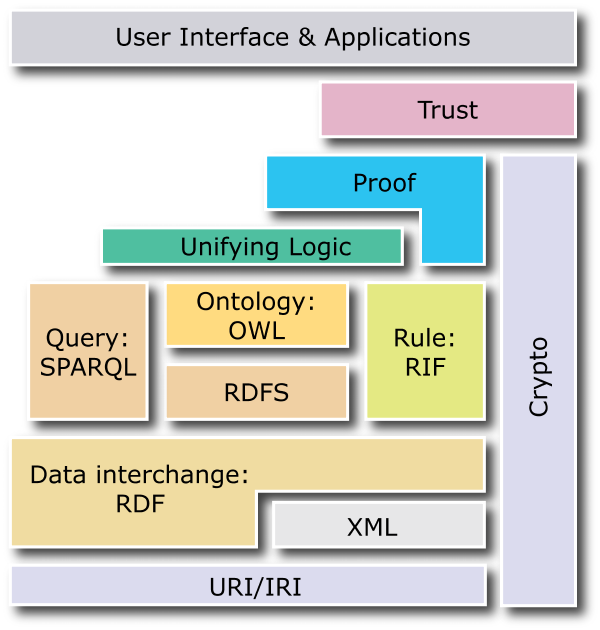
\includegraphics[width=0.8\columnwidth]{images/semantic_web_layers.png}
	\caption[The Semantic Web Model]{The Semantic Web Model \citep{W3C2013}}
\label{fig:images_semweb_model}
\end{figure}

% section semantic_fundamentals (end)

\subsection{A Resource Description Framework}
\label{sec:semantic_rdf}

When trying to come up with a specification on how to integrate data on a globally dispersed platform such as the World-Wide Web, one will have to answer the following questions: \@

\begin{itemize}
	\item \textbf{syntax:} How to serialize the data?
	\item \textbf{data model:} How to structure and organize the data?
	\item \textbf{semantics:} How to interpret the data?
\end{itemize}

Whereas the World-Wide Web is made up from interlinked documents in the \gls{HTML} format that are specifically designed for rendering information on screen, and will be consumed by a human, the \gls{RDF} brings a highly flexible data model to the Web. Its basic building block is the \emph{triple}, that is a statement consisting of an entity, an attribute and a value. The individual parts of a statement are also known as subject, predicate and object, and make up a directed graph as shown in the example in Figure~\ref{fig:images_semweb_triple}: \@

\begin{figure}[H]
	\centering
		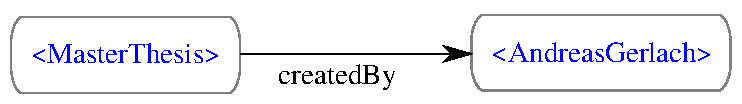
\includegraphics[width=0.8\columnwidth]{images/sample_triple.pdf}
	\caption{A basic example for a triple-statement}
\label{fig:images_semweb_triple}
\end{figure}

In this example the triple consists of the entity ``MasterThesis'', the assigned attribute ``createdBy'' and the value ``AndreasGerlach''. The value-part of a triple can contain either a literal value or refer to another entity (as in the example shown above). Still a problem with this example statement is that the entities are not unique. Based on the given information it is not clear, which specific ``MasterThesis'' is meant and to whom the value ``AndreasGerlach'' refers. Additionally the predicate used can have multiple meanings. These ambiguities have to be resolved on the Semantic Web to be able to make these information understandable by machines. To solve these issues the Semantic Web standard specifies that names of entities and predicates have to use a \gls{URI} (see Section~\ref{subsec:uri_concept}) to make their intended meanings clear. Literals that can be also used as values, such as numbers, dates and strings, borrow their data type specifications from the \gls{XML} standard \citep[pg. 15-38]{wood2014linked}. \\

Based on this description the foundational elements of \gls{RDF} can be summarized as: \@

\begin{itemize}
	\item \textbf{entities:} aka resources or ``things of interest'' that are identified via \gls{URI}s,
	\item \textbf{predicates:} aka attributes or properties that specify the relations between resources and are also identified by \gls{URI}s,
	\item \textbf{literals:} integral values such as numbers, dates and strings that are based on the \gls{XML} data type specification,
	\item \textbf{statements:} assign a value (either another entity or a literal) to a ``entity-predicate'' relation,
	\item \textbf{graphs:} are the data model behind \gls{RDF} and enable a  distributed, interlinked ``Web of Data''.
\end{itemize}

\gls{RDF} triples can be serialized into four different syntax formats \citep[pg. 43-54]{wood2014linked}: \@

\begin{itemize}

	\item \textbf{\gls{RDF}/\gls{XML}:} the original format of the \gls{RDF} data sets is based on the \gls{XML} specification. Because of their complexity they are best used with a parser program. For an example see Listing~\ref{lst:xml_meta_data}.
	\item \textbf{\gls{RDFa}:} describes how to embed \gls{RDF} information into existing \gls{HTML} documents. It allows authors to enrich their Web pages with semantic information by adding a set of predefined \gls{HTML} attributes to important items within the document. Listing~\ref{lst:rdfa_meta_data} shows a basic example.
	\item \textbf{\gls{JSON-LD}:} a recent initiative to allow JavaScript developers to use \gls{JSON} documents to express a \gls{RDF} data set, see Listing~\ref{lst:jsonld_meta_data} for an example.
	\item \textbf{Turtle:} a human readable serialization format for \gls{RDF} statements. \gls{URI}s can be shortened with a predeclared prefix, statements have to be finished with a period. Statements referring to the same entity can be abbreviated via a colon, which repeats the subject from the previous statement, or a comma, which repeats subject and predicate from it. For an example see Listing~\ref{lst:turtle_meta_data}.
\end{itemize}

\begin{listing}[H]
	\begin{minted}[linenos,
	               numbersep=5pt,
	               breaklines=true,
	               frame=lines,
								 gobble=2]{XML}
		<?xml version="1.0"?>
		<rdf:RDF xmlns:rdfs="http://www.w3.org/2000/01/rdf-schema#"
			xmlns:ex="http://www.example.com/">
		  <rdf:Description rdf:about="http://www.example.com/MasterThesis">
		    <ex:createdBy rdf:resource="http://www.example.com/AndreasGerlach" />
		  </rdf:Description>
		</rdf:RDF>
	\end{minted}
\caption{A triple statement expressed in \gls{RDF}/\gls{XML} format}
\label{lst:xml_meta_data}
\end{listing}

\begin{listing}[H]
	\begin{minted}[linenos,
	               numbersep=5pt,
	               breaklines=true,
	               frame=lines,
								 gobble=2]{HTML}
	  <div about="http://www.example.com/MasterThesis">
	    <span rel="http://www.example.com/createdBy" resource="http://www.example.com/AndreasGerlach">
	  </div>
	\end{minted}
\caption{A triple statement expressed in \gls{RDFa} format}
\label{lst:rdfa_meta_data}
\end{listing}

\begin{listing}[H]
	\begin{minted}[linenos,
	               numbersep=5pt,
	               breaklines=true,
	               frame=lines,
								 gobble=2]{JSON}
  {
   "@context": "http://www.example.com/",
   "@id": "http://www.example.com/MasterThesis",
   "createdBy": "http://www.example.com/AndreasGerlach"
 	}
	\end{minted}
\caption{A triple statement expressed in \gls{JSON-LD} format}
\label{lst:jsonld_meta_data}
\end{listing}

\begin{listing}[H]
	\begin{minted}[linenos,
	               numbersep=5pt,
	               breaklines=true,
	               frame=lines,
								 gobble=2]{TURTLE}
	  @prefix ex:  <http://www.example.com/> .
	  ex:MasterThesis ex:createdBy ex:AndreasGerlach .
	\end{minted}
\caption{A triple statement expressed in Turle format}
\label{lst:turtle_meta_data}
\end{listing}

Interestingly, these different serialization formats for \gls{RDF} data sets are fully interchangeable. A \gls{RDF} data set can be easily converted from one serialization format to the other, and merging \gls{RDF} data sets work with sources expressed in different formats as well. \\

Coming back to the initial questions that have to be solved for data integration on Web scale, the section showed how the Semantic Web initiative tries to solve them, such as this: \@

\begin{itemize}
	\item \textbf{syntax:} support for the following formats: Turtle, \gls{RDFa}, \gls{RDF}/\gls{XML} and \gls{JSON-LD},
	\item \textbf{data model:} use the graph-based data model of \gls{RDF},
	\item \textbf{semantics:} express the semantics of the data in \gls{RDFS}. This will be the topic of the next section.
\end{itemize}

% section semantic_rdf (end)

\subsection{\gls{RDF} vocabularies and Web Ontologies}
\label{sec:semantic_vocab_ontologies}

For describing domain specific semantics of the data in a \gls{RDF} data set one can either use the lightweight \gls{RDFS} standard to define available entities and their relationships, or use the more expressive \gls{OWL} specification from the \gls{W3C}. \\

Both specifications are based on the \gls{RDF} data model, and make use of the following predefined \gls{URI}s to declare their meanings, see Table~\ref{tab:w3c_vocab_rdf}: \@

\begin{table}[H]
\centering
\begin{tabular}{p{3cm}llp{4.5cm}}
\hline
\textbf{Name} & \textbf{Prefix} & \textbf{Used for} & \textbf{Namespace URI} \\
\hline
\gls{RDF} & rdf: & Core \gls{RDF} framework & \url{http://www.w3.org/1999/02/22-rdf-syntax-ns\#} \\
\hline
\gls{RDFS} & rdfs: & Define \gls{RDF} vocabularies & \url{http://www.w3.org/2000/01/rdf-schema\#} \\
\hline
Web Ontology Language & owl: & Define ontologies & \url{http://www.w3.org/2002/07/owl\#} \\
\hline
\end{tabular}
\caption[\gls{RDF} vocabularies specified by the \gls{W3C}]{\gls{RDF} vocabularies specified by the \gls{W3C} \citep[pg. 41]{wood2014linked}}
\label{tab:w3c_vocab_rdf}
\end{table}

An important step in the definition of a \gls{RDF} vocabulary or Web ontology is to analyze the domain of interest in detail, and come up with a list of objects and their possible relations. One can use the following step-by-step guide as a reference \citep[pg. 40-55]{antoniou2012semantic}: \@

\begin{enumerate}
	\item Specify the \emph{things} to talk about. These have to be divided into \emph{objects} (aka real entities) and \emph{classes} (aka set of entities). A specific statement containing the predicate ``rdf:type'' assigns individual objects to their classes.
	\item Set up relations that are available between these classes. The relations can either be of type inheritance or composition.
	\item Define existing properties (aka predicates) and their hierarchical relationships (if appropriate).
	\item Impose restrictions on the kind of properties that can be used on objects. These can include restrictions on the \emph{values} a predicate might take (aka ``rdfs:range'' restrictions), and restrictions on the possible \emph{subjects} of a predicate (aka ``rdfs:domain'' restrictions).
\end{enumerate}

The fundamental concepts of the \gls{RDFS} specification, which are used to model entities and their relations within a domain, are listed in Table~\ref{tab:w3c_vocab_rdfs}.

\begin{table}[H]
\centering
\begin{tabular}{p{5cm}p{7cm}}
\hline
\textbf{Classes} & \textbf{Used for} \\
\hline
rdfs:Resource & individual resources \\
\hline
rdfs:Class & classes \\
\hline
rdfs:Literal & literals \\
\hline
rdfs:Propery & properties \\
\hline
\textbf{Predicate} & \textbf{Describes} \\
\hline
rdf:type	& kind of class \\
\hline
rdfs:subClassOf 	&	inheritance between classes \\
\hline
rdfs:subPropertyOf 	& inheritance between properties \\
\hline
rdfs:domain	&	restrict the subjects of a property \\
\hline
rdfs:range  & restrict the values of a property \\
\hline
\end{tabular}
\caption[\gls{RDFS} axioms commonly used to define \gls{RDF} vocabularies]{\gls{RDFS} axioms commonly used to define \gls{RDF} vocabularies \citep[pg. 46-49]{antoniou2012semantic}}
\label{tab:w3c_vocab_rdfs}
\end{table}

As an example the Listing~\ref{lst:sample_rdf_schema} describes a \gls{RDF} data set, which is also displayed in Figure~\ref{fig:images_rdfs_sample}, like that: \@

\begin{enumerate}
	\item there is a class ``Song'' that is derived from the general class ``Audio''
	\item a class of type ``Song'' can have a predicate named ``title''
	\item the predicate ``title'' is a subproperty of ``attribute'' and can contain a literal value
\end{enumerate}

\begin{figure}[H]
	\centering
	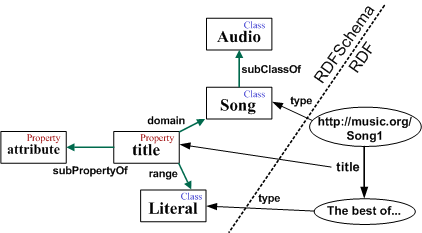
\includegraphics[width=0.9\columnwidth]{images/RDFSchema.png}
	\caption{RDF Schema sample}
	\label{fig:images_rdfs_sample}
\end{figure}

\begin{listing}[H]
  \inputminted[linenos,
               numbersep=5pt,
               breaklines=true,
               frame=lines]{TURTLE}
               {./samples/sample_rdf_schema.ttl}
  \caption{A sample \gls{RDF} data set based on Figure~\ref{fig:images_rdfs_sample}}
\label{lst:sample_rdf_schema}
\end{listing}

As is also shown in Figure~\ref{fig:images_rdfs_sample} the majority of the domain specific knowledge is described in the \gls{RDFS} part of the \gls{RDF} data set. It holds all available classes, predicates, restrictions, \ldots, and is therefore more abstract and expressive. The \gls{RDF} part containing the specific instances might be rather small and concrete, consisting of only existing resources with their known predicates. Usually each of the real entities from the \gls{RDF} part refer to its best matching and most descriptive entity from the \gls{RDFS} part (e.g.\ the entity \url{http://music.org/Song1} in the sample is referring to the \emph{Song} class rather than the \emph{Audio} class). \\

Its important to note that the meaning of the \gls{RDFS} predicates ``rdfs:subClassOf'', ``rdfs:subPropertyOf'' as well as ``rdfs:domain'' and ``rdfs:range'' is \emph{not} to restrict or validate the proper usage of them in a \gls{RDF} statement, but is rather used to \emph{infer} additional statements in a \gls{RDF} data set based on their usage. So in the example above, one can infer that the resource found at \url{http://music.org/Song1} is not only a ``Song'', but also an ``Audio'' based on the ``rdfs:subClassOf'' relationship between ``Song'' and ``Audio''. This kind of propagation of \gls{RDF} statements based on the usages of those \gls{RDFS} predicates fits well to the Open World Assumption of the Semantic Web \citep[pg. 125-152]{allemang2011semantic}. \\

In addition to the axioms shown above the \gls{RDF} and \gls{RDFS} specifications contain further useful entities and predicates, such as shown in Table~\ref{tab:w3c_vocab_supplement}: \@

\begin{table}[H]
\centering
\begin{tabular}{p{5cm}p{7cm}}
\hline
\textbf{Classes} & \textbf{Used for} \\
\hline
rdf:Bag & unordered list of entities \\
\hline
rdf:Seq & ordered list of entities \\
\hline
rdf:Alt & list of alternatives or choices \\
\hline
rdf:Container & superclass of all containers \\
\hline
\textbf{Predicates} & \textbf{Describes} \\
\hline
rdfs:seeAlso &	links to an external resource that contains additional information about it \\
\hline
rdfs:isDefinedBy & links to the original definition of a resource \\
\hline
rdfs:comment & comments and notes on entities \\
\hline
rdfs:label & human friendly label for entities \\
\hline
\end{tabular}
\caption[\gls{RDF} and \gls{RDFS} supplemental axioms]{\gls{RDF} and \gls{RDFS} supplemental axioms \citep[pg. 46-49]{antoniou2012semantic}}
\label{tab:w3c_vocab_supplement}
\end{table}

As the two tables (Table~\ref{tab:w3c_vocab_rdfs} and Table~\ref{tab:w3c_vocab_supplement}) show the \gls{RDFS} specification contains only basic axioms to describe an entity and its possible relationships as well as the hierarchy between these entities and the relations. It is the fundamental set of constraints that is needed to start with publishing resources on the Semantic Web. As of this it does not include more advanced features that can be of use for combining and reasoning on distributed \gls{RDF} data sets, such as: \@

\begin{itemize}
	\item \textbf{Equality/Inequality:} Neither \gls{RDF} nor \gls{RDFS} provide a way to specify that two resources or properties coming from different \gls{RDF} data sets are the same, or are not the same. Though it might be possible to model the aspect of equality with a combination of ``rdfs:subClassOf'' or ``rdfs:subPropertyOf'' statements the results are usually not as desired due to the inferencing nature of those axioms.
	\item \textbf{Cardinality:} Predicates defined in \gls{RDFS} can be used multiple times in statements referring to the same subject or object. This is not desired in situations, in which there is only one possible instance of a ``subject-predicate-object'' relationship.
	\item \textbf{Transitivity:} Whereas it is possible to express the hierarchy of classes and predicates in \gls{RDFS} it is not feasible to do so for individual instances. This might be useful when building up a hierarchy of people, e.g.\ a statement such as ``S3 has an ancestor S2, who has an ancestor S1'' can lead to the inference ``S3 has an ancestor S1''.
	\item \textbf{Property Restrictions:} To define whether a predicate is referring to an object or a literal as value is not possible with \gls{RDFS}, but may be useful for modeling and editing tools.
\end{itemize}

Therefore, in case there is more expressiveness required to model a domain one can use additional concepts from the Web Ontology Language specification (\gls{OWL}). It is build on the \gls{RDFS} specification, but contains additional constraints and classifiers, some of the most commonly used ones are listed in Table~\ref{tab:w3c_vocab_owl}. \@

\begin{table}[H]
\centering
\begin{tabular}{p{5cm}p{7cm}}
\hline
\textbf{Classes} & \textbf{Used for} \\
\hline
owl:Class & all classes in \gls{OWL}  \\
\hline
owl:FunctionalProperty & allow only one value \\
\hline
owl:InverseFunctionalProperty & allow only one source \\
\hline
owl:TransitiveProperty & build chains of relationships \\
\hline
owl:ObjectProperty & property can hold a resource as value \\
\hline
owl:DataProperty & property can hold a literal as value \\
\hline
\textbf{Predicates} & \textbf{Describes} \\
\hline
owl:equivalentClass &	equality of classes \\
\hline
owl:equivalentProperty & equality of properties \\
\hline
owl:sameAs & equality of individual resources \\
\hline
\end{tabular}
\caption[Commonly used \gls{OWL} axioms]{Commonly used \gls{OWL} axioms \citep[pg. 153-185]{allemang2011semantic}}
\label{tab:w3c_vocab_owl}
\end{table}

The Table~\ref{tab:w3c_vocab_owl} is only showing a small subset of the axioms available in \gls{OWL}. The Web Ontology Language can be used to express a wide variety of constraints and classifiers on predicates, and the whole specification is based on three parts that are build upon each other \citep{owlspec}. Still, with an increase of expressiveness in the model the complexity of the reasoning and inferencing engine also grows up, because most of these axioms are used to express inferences that can be drawn on the \gls{RDF} data set. This Master thesis is restricting the usage of axioms of the \gls{OWL} specifications to ones shown in Table~\ref{tab:w3c_vocab_owl}.

% section semantic_ontologies (end)

\subsection{\gls{SPARQL} protocol and query language}
\label{sec:semantic_querylang}

A kind of query language is required to be able to access specific information in a \gls{RDF} data set on the Semantic Web. Additionally, the query language has to support the distributed nature of information on the Semantic Web, as well as be suitable for asking information from the graph-oriented data model of \gls{RDF}. The \gls{W3C} proposes the \gls{SPARQL} protocol and query language as a standard way to access and query for information on the Semantic Web. As the name already implies the specification contains two parts: a \emph{protocol} and a \emph{query language}. \\

\gls{SPARQL} requires the \gls{RDF} data set in a \emph{triple store}, which is a kind of database containing \gls{RDF} statements (another name for it might be \emph{graph store}). The \gls{RDF} data set is usually inserted into the triple store via bulk load operations or single \gls{SPARQL} update statements, which like in \gls{SQL} for relational databases can manipulate \gls{RDF} statements in the data store. A \gls{SPARQL} query is usually expressed in a Turtle-like syntax and is send to an \gls{HTTP} endpoint of the triple store by a client application. The result of the query can contain either a single value, a tabular data stream, or a subgraph of the \gls{RDF} data set depending on the type of query issued. The structure of a Semantic Web application that uses a triple store (aka \gls{RDF} store) and the \gls{SPARQL} query engine is depicted in Figure~\ref{fig:images_semweb_app} \citep[pg. 51-60]{allemang2011semantic}:

\begin{figure}[H]
	\centering
	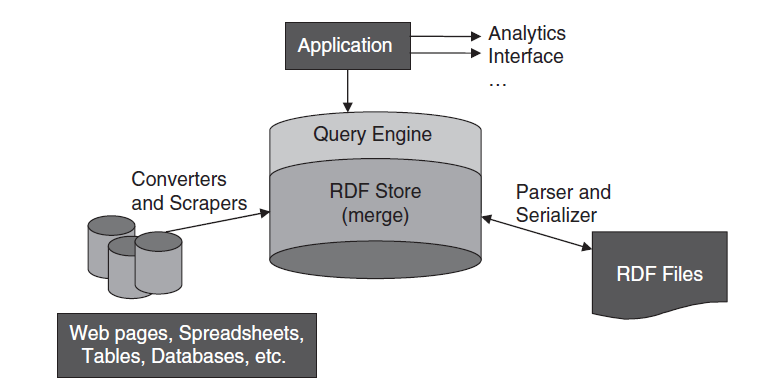
\includegraphics[width=0.9\columnwidth]{images/semantic_web_application.png}
	\caption[Semantic Web application architecture]{Semantic Web application architecture \citep[pg. 57]{allemang2011semantic}}
	\label{fig:images_semweb_app}
\end{figure}

The \gls{SPARQL} query language has a lot of similarities with the \gls{SQL} used for querying relational databases. This design decision will ease the transition to the Semantic Web for application developers familiar with accessing data from a relational database. The main difference though is the way used to specify the conditions for a query. This is largely due to the differences in the underlying data model, which is relational in \gls{SQL} versus graph-oriented in \gls{SPARQL}. As of this, a WHERE clause in a \gls{SPARQL} query has to contain a graph-based representation of the query conditions that have to be matched in the \gls{RDF} data set. Parts of these conditions can be marked as placeholders, which are referred to in a SELECT statement for generating a tabular data output. These placeholders are marked with a question-mark in the beginning of their name and can be used as placeholder for any part of a triple statement (subject, predicate, object) \citep[pg. 66-112]{allemang2011semantic}. E.g.\ querying a \gls{RDF} data set containing triples such as the one described in Listing~\ref{lst:sample_rdf_schema} for the titles of all available songs, one has to write a \gls{SPARQL} SELECT query as shown in Listing~\ref{lst:select_sparql}: \@

\begin{listing}[H]
	\inputminted[linenos,
							 numbersep=5pt,
							 breaklines=true,
							 frame=lines]{SPARQL}
							 {./samples/sample_sparql_select.sparql}
\caption{Selecting the title from all songs with \gls{SPARQL}}
\label{lst:select_sparql}
\end{listing}

Please note that this query defines two placeholders in the WHERE clause: ``?song'' and ``?title'', but only uses the ``?title'' as an output criteria in the SELECT statement. The placeholder ``?song'' is \emph{just} required to refer to the same node when specifying the conditions in the WHERE clauses. \\

The WHERE clause in a \gls{SPARQL} query can include additional conditions that have an effect on the returned information, such as \citep[pg. 66-112]{allemang2011semantic}: \@

\begin{itemize}
	\item \textbf{LIMIT:} specifies the upper limit of results that should be returned from a \gls{SPARQL} query; e.g.\ LIMIT 100
	\item \textbf{FILTER:} express additional filter conditions on the result set of a \gls{SPARQL} query; e.g.\ FILTER(?releaseDate \textgreater ``1980-01-01'')
	\item \textbf{UNION:} combine the result sets from different graph patterns into one; e.g.\ \{ ex:Song ex:title ``A'' \} UNION \{ ex:Song ex:title ``G'' \}
\end{itemize}

Beside the SELECT statement, that returns tabular data, \gls{SPARQL} also supports the ASK type of query, which checks for the existence of graph patterns stated in the WHERE clause, and will return a boolean value (true or false). This kind of query is commonly used to assert the presence of certain triples in a \gls{RDF} data set. \\

Another kind of query is the CONSTRUCT statement, that is used to retrieve a subgraph from a \gls{RDF} data set, and can also be used to harmonize graphs from different sources, that use different schemata. As a query of type CONSTRUCT will return a new \gls{RDF} graph it can also be used for basic reasoning functionality ala ``if this graph-pattern is found, assume that \ldots'', as well as to help with resolving issues of identifying entities that are described with different \gls{URI}s \citep[pg. 88-98]{allemang2011semantic}.
E.g.\ querying a \gls{RDF} data set containing triples such as the one described in Listing~\ref{lst:sample_rdf_schema} and mapping the song information to the DublinCore specification \citep{DublinCore}, one has to write a \gls{SPARQL} CONSTRUCT query as shown in Listing~\ref{lst:construct_sparql}. \\

\begin{listing}[!ht]
	\inputminted[linenos,
							 numbersep=5pt,
							 breaklines=true,
							 frame=lines]{SPARQL}
							 {./samples/sample_sparql_construct.sparql}
\caption{Mapping custom song information to the DublinCore vocabulary with \gls{SPARQL}}
\label{lst:construct_sparql}
\end{listing}

Please note that the CONSTRUCT statement consists of a set of triple statements that will make up the resulting \gls{RDF} graph.

% section semantic_querylang (end)

% section semantic_web (end)
